
%----------------------------------------------------------------------------------------
%	Lecture 2
%----------------------------------------------------------------------------------------

\section*{\centering Limits \& Continuity}

\bigbreak
\section{Continuity}

We say $f(x)$ is continuous at $x_0$ when

\begin{equation*}
\lim_{x \to x_0} f(x) = f(x_0)
\end{equation*}

\subsection*{Two Trig Limits}

Note : In the expression below, $\theta$ is in radians --- NOT degrees.

\begin{equation*}
\boxed{
	\lim_{\theta \to 0} \frac{\sin \theta}{\theta} = 1; \quad \lim_{\theta \to 0} \frac{1-\cos \theta}{\theta} = 0
}
\end{equation*}

Here is a geometric proof of the first limit : 

\begin{figure}[h]
	\centering
	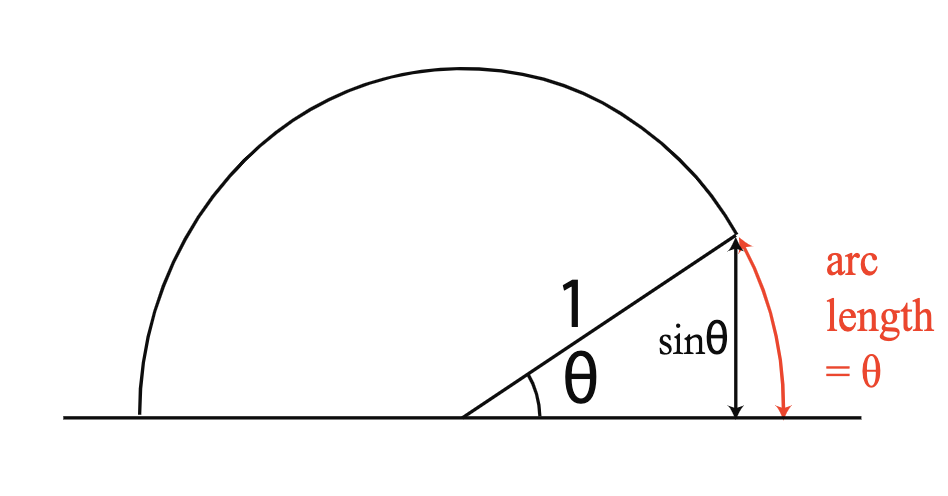
\includegraphics[scale=0.7]{./images/lecture_2_figure_1.png}
	\caption{A circle with radius 1 with an arc of $\theta$}    
\end{figure}

\begin{figure}[h]
	\centering
	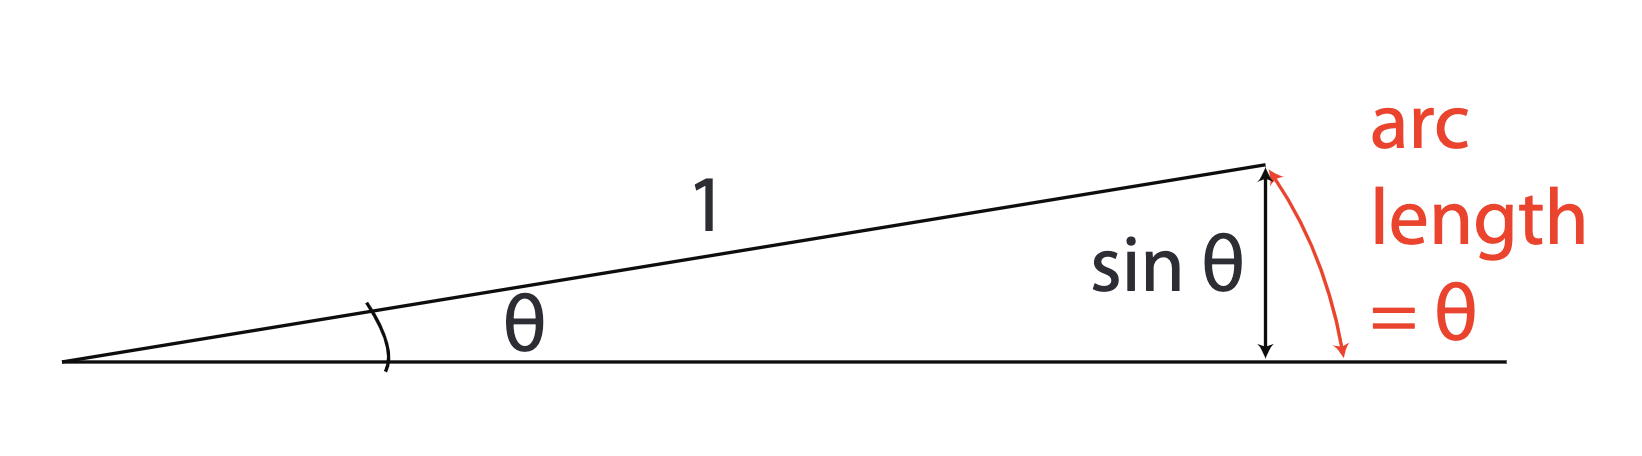
\includegraphics[scale=0.5]{./images/lecture_2_figure_2.png}
	\caption{A circle with radius 1 with an arc of $\theta$}    
\end{figure}

Imagine what happens to the picture as $\theta$ gets very small.
As $\theta \to 0$, we see that $\frac{\sin \theta}{\theta} \to 1$.

\pagebreak

What about the second limit involving cosine?

\begin{figure}[h]
	\centering
	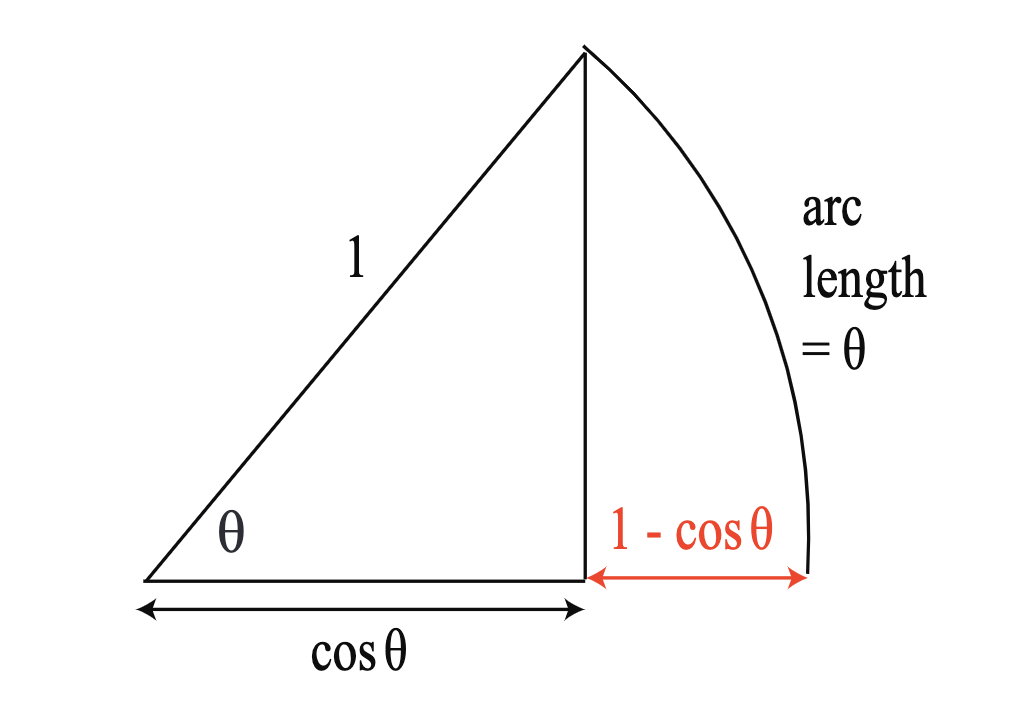
\includegraphics[scale=0.5]{./images/lecture_2_figure_3.png}
	\caption{Same as Fig. 4 except that the horizontal distance is marked.}    
\end{figure}


From above figure, we can see that as $\theta \to 0$, the length of $1-\cos \theta$ of the short segment gets much smaller than the vertical distance $\theta$ along the arc.
Hence, $\frac{1-\cos \theta}{\theta} \to 0$ 


\begin{figure}[h]
	\centering
	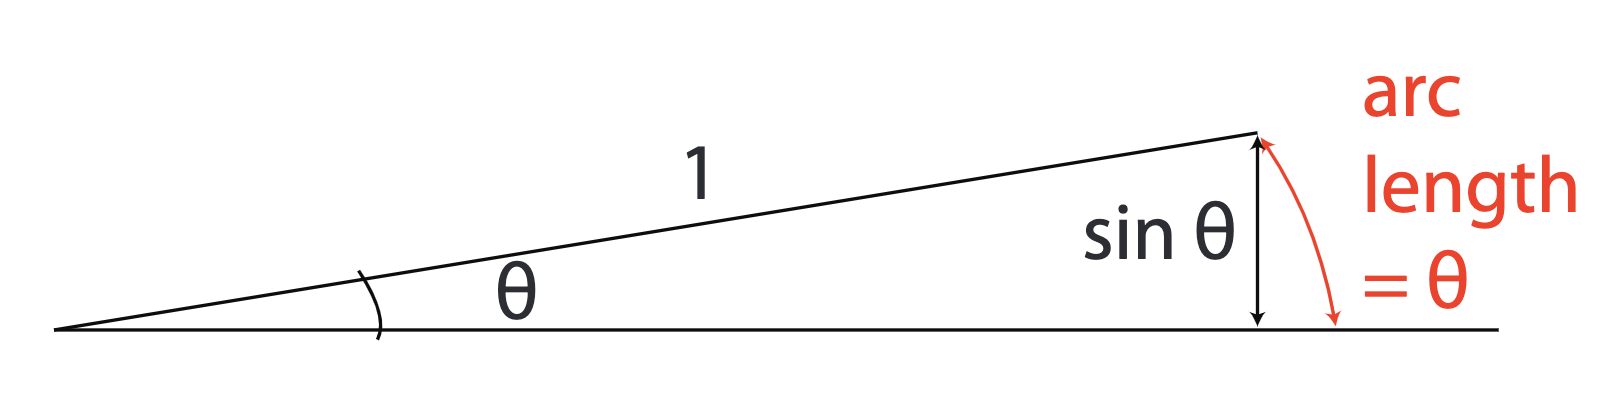
\includegraphics[scale=0.5]{./images/lecture_2_figure_4.png}
	\caption{The sector in Fig. 5 as it $\theta$ becomes very small.}    
\end{figure}

\subsection*{Theorem : Differentiable Implies Continuous}
If $f$ is differentiable at $x_0$, then $f$ is continuous at $x_0$.

\subsubsection*{Proof:} 

\begin{equation*}
\lim_{x \to x_0} \left( f(x) - f(x_0) \right)
	= \lim_{x \to x_0} \left[ \frac{f(x) - f(x_0)}{x-x_0} \right] (x - x_0) = f`(x-x_0) \cdot 0 = 0 
\end{equation*}
